% !TEX root = sum1.tex
\section{Problem Description}
In this section, we first consider the seat planning problem with social distance. Then we introduce the dynamic seat assignment problem with social distance.

% Then we incorporate the social distance into seat planning.

% give the description of the seat planning problem with social distance.

% dynamic seat assignment problem, which is suitable for commercial use in cinemas and concerts.


\subsection{Seat Planning Problem with Social Distance}\label{dynamic_demand}
We consider a set of groups, each of which consists of no more than $m$ people, to be assigned to a set of seats. There are $m$ different group types, with group type $i$ having a size of $s_i$, where $1 \leq i \leq m$. These groups can be represented by a demand vector, denoted by $\mathbf{d} = (d_1, \ldots, d_m)$. Each element $d_i$, where $1 \leq i \leq m$, indicates the number of group type $i$ containing $i$ people. For illustration, we consider a layout consisting of $N$ rows, each containing $S_j$ seats, where $j = 1, \ldots, N$.

In accordance with epidemic prevention requirements, customers from the same group are allowed to sit together, while different groups must maintain social distancing which can be one seat or more seats. We consider the social distance of one empty seat throughout the rest of this paper, which is more practical and reasonable in the seat planning. However, our methods are still applicable to the social distance of two or more seats.

Specifically, each group must leave one seat empty to maintain social distancing from adjacent groups. Additionally, different rows do not affect each other, meaning that a person from one group can sit directly behind a person from another group.

To achieve the social distancing requirements in the seat planning process, we add one to the original size of each group to create the new size of the group. We also add one dummy seat to each row. Let $s_i = i + 1$ denote the new size of group type $i$, and let $L_j = S_j + 1$ denote the length of row $j$, where $S_j$ represents the number of seats in row $j$.

Then we can illustrate the seat planning for one row below. 

\begin{figure}[ht]
    \centering
    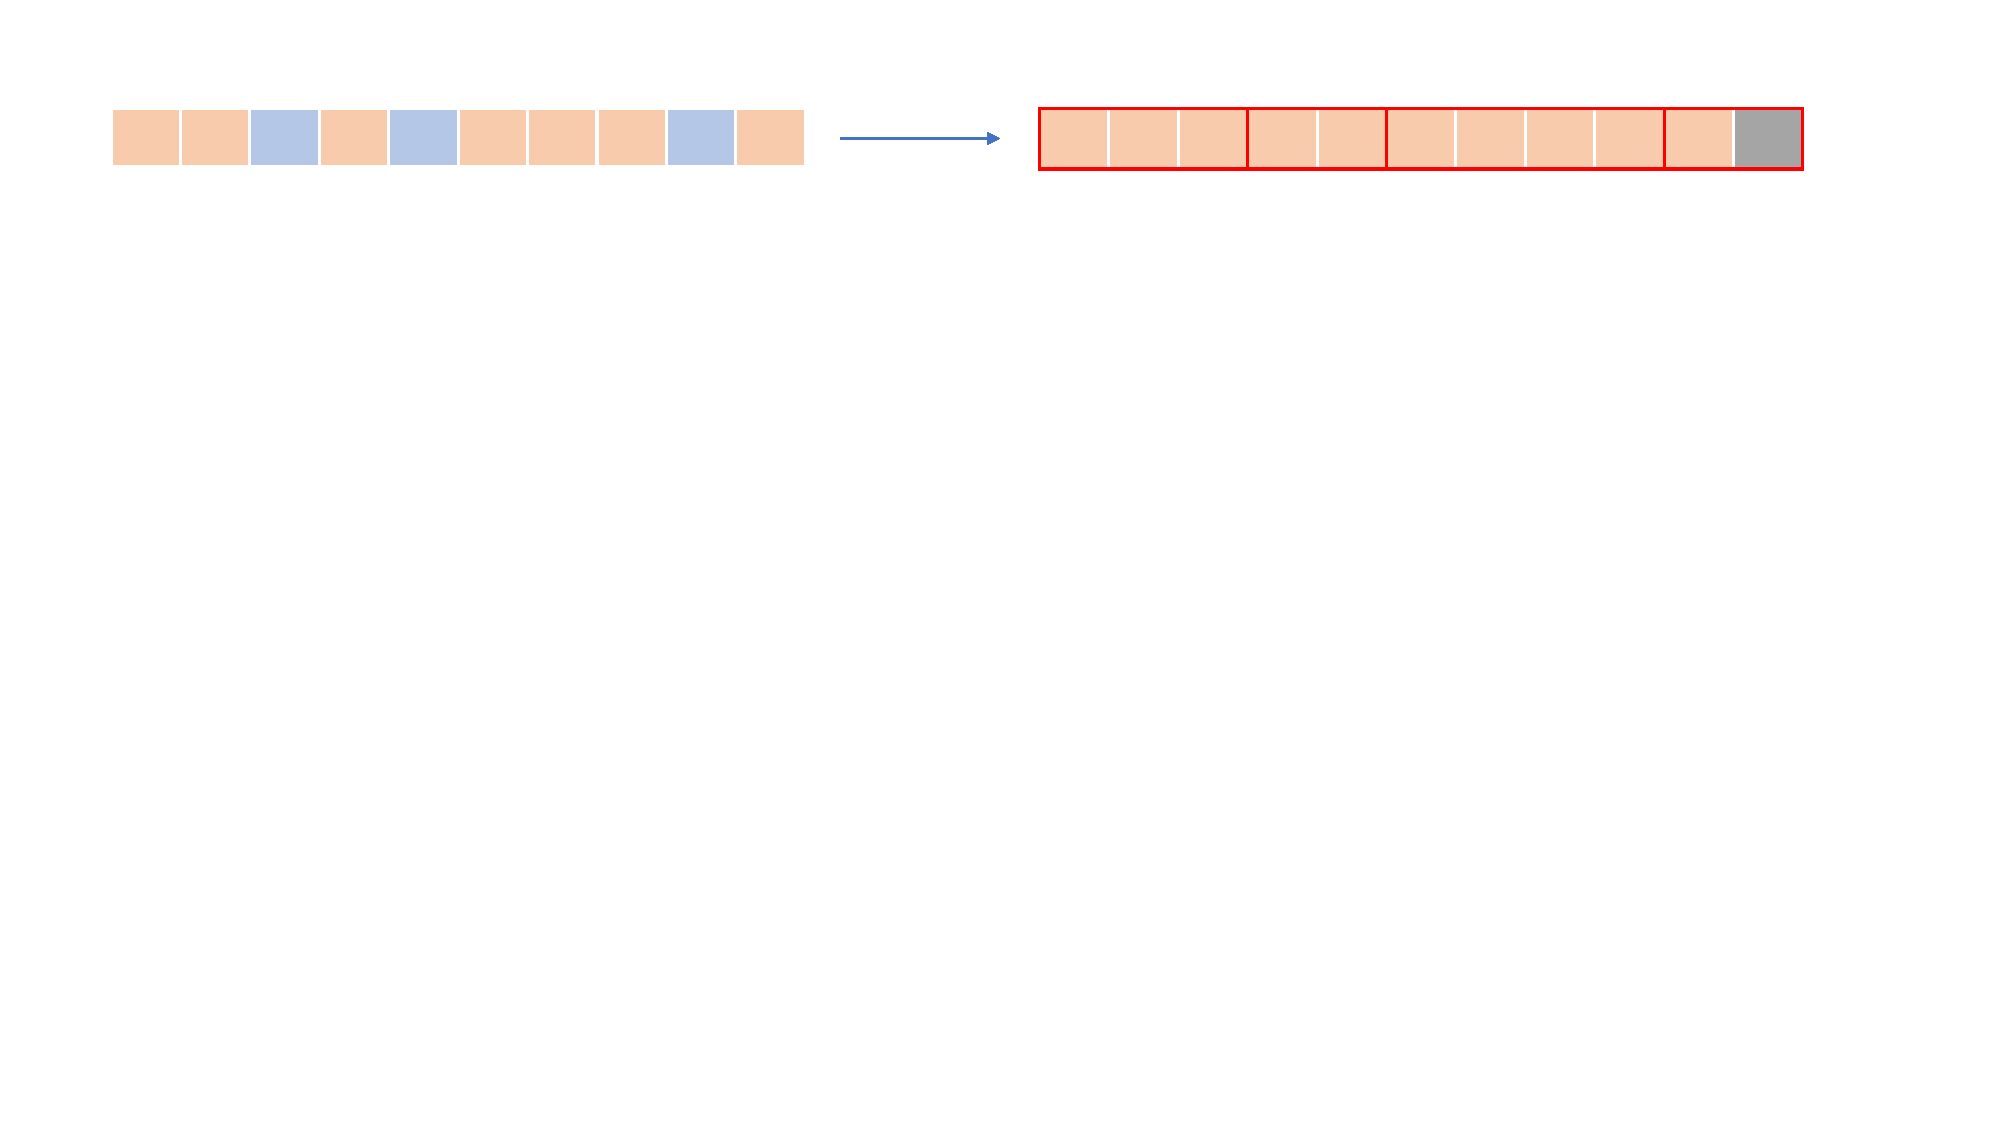
\includegraphics[width = 0.8\textwidth]{./Figures/dummy_seat.pdf}
    \caption{Problem Conversion}
\end{figure}


On the left side of the diagram, the blue squares represent the empty seats required for social distancing, while the orange squares represent the seats occupied by groups. On the right side, we have added one dummy seat at the end of each row. The orange squares surrounded by the red line represent the seats taken by groups in this row, which includes two groups of 1, one group of 2, and one group of 3.

By incorporating these additional seats and designating certain seats for social distancing, we can integrate social distancing measures into the seat planning problem.

% As stated above, we can obtain such a seating plan from stochastic programming. However, it only gives the initial seat assignment without handling the dynamic situation. 


\subsection{Dynamic Seat Assignment with Social Distance}
% In this section we present the model that generates seat planning under deterministic demands.

% Let the $i-$th group type contain $i$ people. 
% $(d_1, d_2, d_3, d_4) = (3,5,7,6)$

% But our model and formulation allow for a more general layout of the seats. 
Now consider the scenario where groups arrive dynamically, the decision-maker must determine whether to accept or reject each group and assign them to empty seats while ensuring that the social distancing constraint is met. Once the seats are confirmed and assigned to a group, they cannot be changed.

We use a vector $\mathbf{S}= (S^{r}_1, S^{r}_2, \ldots, S^{r}_{N})$ to record the remaining capacity of rows, where $S^{r}_{j}$ represents the number of remaining seats in row $j$. Let $V_{t}(\mathbf{S})$ denote the maximal expected value to go at period $t$ with capacity of rows. Let $\mathbf{w} = (s_1+1, \ldots, s_m+1)$ be the number of seats occupied by each group type. There are $T$ periods and the arrival probability of the group type $i$ in each period is $p_i$. In every period, the group can decide which row to sit.

The dynamic programming formulation for this problem is
$$V_{t}(\mathbf{S}) = E_{p_i} \left[ \max_{k \in N: S_k \geq s_i +1} \{ {[V_{t-1}(\mathbf{S}- (\mathbf{w} \circ \mathbf{e}_{i})U_{k})+ s_i]}, {V_{t-1}(\mathbf{S})}\} \right], \mathbf{S} \geq \mathbf{0}, V_{T+1}(\mathbf{S}) = 0,$$

where $\mathbf{e}_{i}$ is the unit vector whose i-th element is 1. $U_k$ is a matrix of $m$ by $n$ with all elements in column $k$ being 1. $\circ$ is the element-wise product. Initially, we have $\mathbf{S}_{T} = (S_1, S_2, \ldots, S_{N})$. 


As we can observe, the dynamic programming algorithm has to make a decision on which row to assign group type $i$. This leads to the curse of dimensionality due to the numerous seating plan combinations. To avoid this complexity, we propose an approach that directly targets the final seating plan and then formulates a policy for assigning groups.

To obtain the final seat planning firstly, we develop the scenario-based stochastic programming.

% The number of all seats in each row is called the length of the row.

% when the capacity allows accepting the groups from large to small as many as possible will give an optimal solution.


% Why is it easy to solve this IP?

% If the ratio is the same for the groups, IP will use more branches to obtain an optimal solution.

% $[24,28,8,9]$ 10 rows.
% Total loss: 60; loss of the largest pattern: 5.


% Specifically, we define the concept of target seating plans deemed satisfactory. In making the dynamic seating plan, we will try to maintain the possibility of achieving one of the target seating plans as much as possible.
